\documentclass[a4paper,12pt,fleqn]{article}
%\usepackage {psfig,epsfig} % para incluir figuras em PostScript
\usepackage{amsfonts,amsthm,amsopn,amssymb,latexsym,subcaption}
\usepackage{graphicx}
\usepackage[T1]{fontenc}
\usepackage[brazil]{babel}
\usepackage{geometry}
\usepackage[utf8]{inputenc}
\usepackage[intlimits]{amsmath}
%alguns macros
\newcommand{\R}{\ensuremath{\mathbb{R}}}
\newcommand{\Rn}{{\ensuremath{\mathbb{R}}}^{n}}
\newcommand{\Rm}{{\ensuremath{\mathbb{R}}}^{m}}
\newcommand{\Rmn}{{\ensuremath{\mathbb{R}}}^{{m}\times{n}}}
\newcommand{\contcaption}[1]{\vspace*{-0.6\baselineskip}\begin{center}#1\end{center}\vspace*{-0.6\baselineskip}}
%=======================================================================
% Dimensões da página
\usepackage{a4}                       % tamanho da página
\setlength{\textwidth}{16.0cm}        % largura do texto
\setlength{\textheight}{9.0in}        % tamanho do texto (sem head, etc)
\renewcommand{\baselinestretch}{1.15} % espaçamento entrelinhas
\addtolength{\topmargin}{-1cm}        % espaço entre o head e a margem
\setlength{\oddsidemargin}{-0.1cm}    % espaço entre o texto e a margem
       
% Ser indulgente no preenchimento das linhas
\sloppy
 

\begin{document}


\pagestyle {empty}

%\input logo

%\vspace*{-3cm}

%\begin{figure}[h]
%\leavevmode
%\begin{minipage}[t]{\textwidth}
%\includegraphics[1cm,1cm][3cm,3cm]{logo-ufrpe.bmp}
%\end{minipage}
%\end{figure}



\vspace*{-2cm}
{\bf
\begin{center}
{\large
\hspace*{0cm}Universidade de São Paulo} \\
\hspace*{0cm}Instituto de Matemática e Estatística \\
\hspace*{0cm}MAC 5742 - Computação Paralela e Distribuída  \\
\end{center}}
\vspace{4.0cm}
\noindent
\begin{center}
{\Large \bf Exercício Programa 1: OpenMP} \\[3cm]
{\Large Autores:}\\[6mm]
{\Large Diana Naranjo}\\[6mm]
{\Large Walter Perez}\\[6mm]
\end{center}




\vspace{8cm}
{\center São Paulo \\[3mm]
Abril 2015 \\}


\newpage


  
\pagestyle {empty}
\abstract{Nesse Exercício Programa (EP) o objetivo foi explorar a computação paralela com memoria compartilhada, para isso foi usado o padrão OpenMP.
A primeira parte do trabalho explora o cuidado que deve-se ter no momento de realizar o desenvolvimento de programas usando as diretivas do OpenMP. É muito simples cometer erros quando ainda se está pensando de maneira sequencial, ao assumir algum comportamento ou quando não se conhece bem o comportamento padrão das diretivas usadas.
A segunda parte do EP procura avaliar as melhoras (ou falta delas) no tempo de execução de um programa alvo, mult.c, que realiza a multiplicação de 2 matrizes. Para avaliar o desempenho da versão sequencial versus a paralela uma serie de experimentos foram realizados. Alguns deles involucraram a alteração do programa para criar distintas zonas paralelas e também a execução deles usando diferentes números de threads.
A continuação presentamos os experimentos, resultados e conclusões.}

\newpage 
 
\tableofcontents 
 
 
% Numeração em romanos para páginas iniciais (sumários, listas, etc) 
%\pagenumbering {roman} 
\pagestyle {plain} 
 
 
 
\setcounter{page}{0} \pagenumbering{arabic} 
 
 
 
 
 
 
  
\setlength{\parindent}{0in}  %espaço entre paragrafo e margem 
% Espaçamento entre parágrafos 
\parskip 5pt   
 \clearpage 
 
\section{Introdução} 
A computação paralela consiste em executar um conjunto de cálculos de maneira simultânea ~\cite{Gottlieb89}. A meta de este tipo de computação é diminuir o tempo de execução que exigem algumas aplicações, e.g. aquelas com fortes requerimentos de computo. Atualmente, existem computadores com múltiplos cores; além de isso também contam com tecnologias como hyper-threading, o que gera que o sistema operativo assuma que conta com uma maior quantidade de recursos de computo. Os recursos, por tanto, estão prontos para ser usados. Porém, para realmente obter uma melhoria no rendimento não é suficiente executar as aplicações em uma máquina multicore, é necessário que elas troquem seus algoritmos sequências por uma versão paralela. De outra maneira, não estaria-se fazendo uso do processamento paralelo e seus benefícios.  

O grande problema é que a troca de algoritmos sequências por paralelos não é um trabalho simples. Existem diversos problemas na geração de códigos paralelos de bom rendimento, alguns deles são ~\cite{Matloff14}: 
\begin{itemize} 
\item Gargalos de comunicação. Debe ter-se em consideração a quantidade processadores que serão utilizados na execução e o overhead produto da comunicação entre estes processadores e a memoria~\cite{Gebali11}. Isto é importante pois pode acontecer que um programa em versão paralela tome mais tempo na execução do que na versão sequencial. O que se debe a que a memoria só pode ser acessada por um thread em qualquer momento e o custo de manter as caches de cada processador coerente também gera um overhead. 
\item Balanceamento de carga. Ao fazer uma divisão de trabalho o ideal é que cada uma das partes tenha uma carga igual. Se uma delas tem mais trabalho do que as outras então no final o problema volta a ser sequencial pois a maioria termina com sua carga e umas poucas continuam com o resto do trabalho. 
\item Problemas na construção do código. Os desenvolvedores estão acostumados a pensar em forma sequencial e por tanto é muito fácil cometer erros de 
concorrência. As operações simples, como por exemplo a assinação de valores a uma variável, causam resultados inesperados na versão paralela. Isto é devido as condições de corrida, i.e. quando o programa se desenvolve em um ordem diferente ao que o programador planeio. 
\end{itemize} 
 Para evitar os erros produzidos por o pouco cuidado do desenvolvedor e para maximizar o paralelismo dos algoritmos que são sequências existem conjuntos de diretivas que criam um código paralelo executável. OpenMP é um conjunto de diretivas para o compilar, rutinas de libraria e variáveis de entorno que podem ser usadas para a geração de paralelismo em códigos Fortran e C/C++ ~\cite{OpenMP13}. O objetivo é garantir o correto funcionamento dos programas e obter os benefícios do paralelismo. 
 
Neste trabalho exploramos os problemas persistentes no uso das diretivas do OpenMP. Tanto no desenvolvimento de código errôneo, como na geração de overhead pela geração de áreas paralelas ineficientes. Para isso desenvolvemos experimentos para obter o tempo promédio na execução de códigos gerados a partir de distintas áreas paralelas, em ambientes diferentes e com distintas quantidades de threads.  
 
\section{Exercício 1} 
\textbf{Escolher um código na internet que use as diretivas de compilação do OpenMP, esse código deve ser procurado nos respetivos tutoriais e manuais desse padrão de programação multiprocessamento. A ideia e encontrar erros nessas implementações fornecidas ou apresentadas nos tutoriais consultados. Apresente o código, aponte os problemas e descreva quais são as correções feitas para tirar o erro da aplicação.} 
 
\subsection{Código com erro} 
Comando para preservar a formatação do texto. 
\begin{verbatim} 
INSERT CODE HERE 
\end{verbatim} 
 
\subsection{Problemas encontrados} 
 
\subsection{Correções} 
Comando para preservar a formatação do texto. 
\begin{verbatim} 
INSERT CODE HERE 
\end{verbatim} 
 
\subsection{Conclusões} 
 
\clearpage 
 \section{Exercício 2} 
\label{sec:tab} 
\textbf{Modifique o programa mult.c, que realiza a multiplicação de 2 matrizes. Modifique este código para que ele realize a multiplicação utilizando as primitivas de paralelização de OpenMP. Compare o desempenho com 1, 2, 3 4, 8 e 16 threads. Tente realizar a paralelização no laço for das variáveis i, j e k, explicando no relatório se o comportamento obtido está correto ou não. Apresente e descreva no relatório grafos, tabelas e estatísticas dos tempos de execução.
\begin{itemize} 
\item Compare o desempenho obtido, explicando por que melhorou ou piorou e compare também a execução do programa em sua versão sequencial. 
\item Um dos objetivos e verificar se algum overhead e inserido pelo ambiente de execução (runtime OpenMP) quando a versão paralela do programa em OpenMP executa apenas com uma (1) thread, comparando-se com a versão sequencial (mult.c). 
\item Esse programa deve ser executado em pelo menos dois processadores diferentes, para efeitos de encontrar os intervalos de confiança cada execução deve ser repetida pelo menos 10 vezes. 
\item Outras informações que julgarem pertinentes ao contexto do trabalho podem ser adicionadas, e poderão ser somadas como pontos adicionais do EP.
\end{itemize}
}
\subsection{Experimentos} 
Os experimentos realizados neste exercício podem ser separados em duas categorias: a primeira consta da adição de diretivas OpenMP para criar as zonas paralelas, a segunda consta tanto da adição das  diretivas como de câmbios no mesmo código para otimizar o uso dos recursos. Cada uma de estas categorias conta com 4 programas diferentes: o programa sequencial, o programa com paralelização no laço da variável $i$, o programa com paralelização no laço da variável $j$, e finalmente, o programa com paralelização no laço da variável $k$. Cada programa, a excepção do programa sequencial, foi executado com diferentes números de threads.  
 
Algumas das características importantes dos experimentos são: 
\begin{itemize} 
    \item Otimização de código. Certas partes do programa original mult.c foram cambiadas para melhorar o uso dos recursos. Estas otimizações foram dois: 
    \begin{itemize}
        \item Variável temporal. Uma variável temporal, $tmp$, foi criada para armazenar a suma das multiplicações no laço $k$.
        \item Método de transposição. Um método de transposição foi implementado para obter um acesso sequencial da matriz $b$ no laço $k$.
    \end{itemize}
    \item Zonas paralelas. Diferentes zonas foram criadas nos laços das variáveis $i$, $j$ e $k$.  
    \item Número de threads. O desempenho foi avaliado com 1, 2, 3, 4, 8 e 16 threads.   
    \item Processadores. Foram utilizados o: \textbf{Intel CoreTM i5-3317U CPU @ 1.70GHz x 4} e o \textbf{Intel Xeon CPU E5-2630L v2 @ 2.40GHz}.
\end{itemize} 

O código de cada um dos experimentos pode ser observado no Anexo 1 e 2. Sendo o Anexo 1 o conjunto de códigos com adições de diretivas de paralelização; e o Anexo 2 os códigos com diretivas de paralelização, além das otimizações mencionadas previamente.  

\subsection{Resultados} 

Os resultados nos tempos de execução dos experimentos da primeira categoria, foram os seguentes: 

\begin{table}[!htb]
    \begin{subtable}{.5\linewidth}
        \centering{
        \resizebox{.9\columnwidth}{!}{%
        \begin{tabular}{|c|r|r|r|r|} \hline
            \multicolumn{1}{|c|}{{\# Threads}} & \multicolumn{1}{|c|}       {{Sequencial}} & \multicolumn{1}{|c|}{{Paralela $i$}} & \multicolumn{1}{|c|}{{Paralela $j$}} & \multicolumn{1}{|c|}{{Paralela $k$}} \\ \cline{1-5}
            1    & 1.4042 & 0.7065  & 0.7559  & 0.7025  \\\hline
            2    & 1.4042 & 0.7169  & 0.7603  & 0.6920  \\\hline
            3    & 1.4042 & 0.7171  & 0.7662  & 0.7268  \\\hline
            4    & 1.4042 & 0.7137  & 0.7616  & 0.6976  \\\hline
            8    & 1.4042 & 0.7074  & 0.7573  & 0.7060  \\\hline
            16   & 1.4042 & 0.7129  & 0.7566  & 0.6960  \\\hline
        \end{tabular}%%
        }}
        \label{tab:corei5so}
        \caption{Intel Core i5}
    \end{subtable}%
    \begin{subtable}{.5\linewidth}
        \centering{
        \resizebox{.9\columnwidth}{!}{%
        \begin{tabular}{|c|r|r|r|r|} \hline
            \multicolumn{1}{|c|}{{\# Threads}} & \multicolumn{1}{|c|}{{Sequencial}} & \multicolumn{1}{|c|}{{Paralela $i$}} & \multicolumn{1}{|c|}{{Paralela $j$}} & \multicolumn{1}{|c|}{{Paralela $k$}} \\ \cline{1-5}
            1    & 2.3469 & 1.2561  & 1.2747  & 0.6990  \\\hline
            2    & 2.3469 & 1.1427  & 1.1572  & 0.6424  \\\hline
            3    & 2.3469 & 1.1389  & 1.1804  & 0.6402  \\\hline
            4    & 2.3469 & 1.2746  & 1.1563  & 0.8217  \\\hline
            8    & 2.3469 & 1.1286  & 1.1179  & 0.7177  \\\hline
            16   & 2.3469 & 1.1921  & 1.1979  & 0.6943  \\\hline
        \end{tabular}%
        }}
        \label{tab:xeonso}
        \caption{Intel Xeon}
    \end{subtable}
    \caption{Diretivas OpenMP, sem Otimizações}
    \label{tab:so}
\end{table}

Os grafos dos tempos de execução podem ser observado nas figuras ~\ref{fig:corei5so} e ~\ref{fig:xeonso}.
 
\begin{figure}[htb] 
    \centering
    \begin{subfigure}{.5\textwidth}
        \centering
        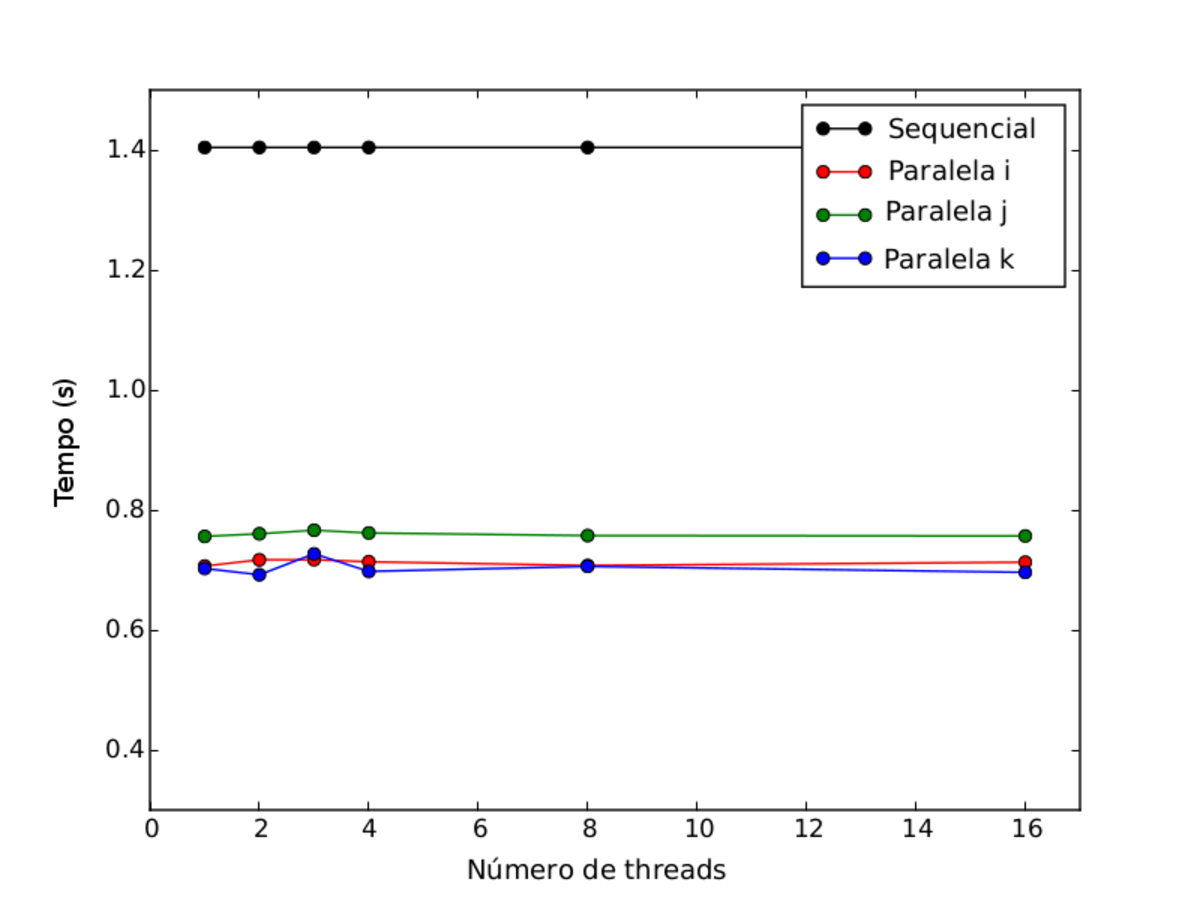
\includegraphics[height=6cm]{Images/corei5so} 
        \caption{Intel Core i5}
        \label{fig:corei5so} 
    \end{subfigure}%
    \begin{subfigure}{.5\textwidth}
        \centering
        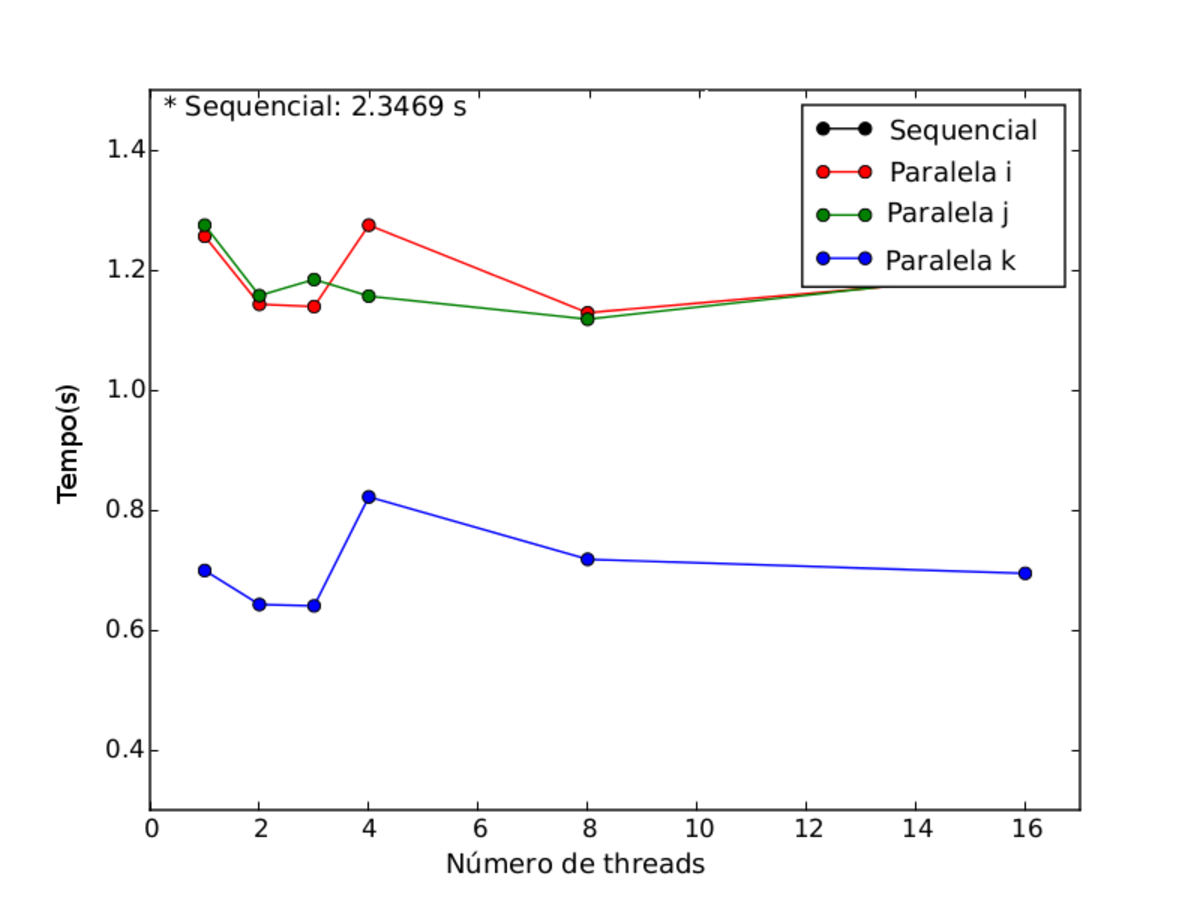
\includegraphics[height=6cm]{Images/xeonso} 
        \caption{Intel Xeon}
        \label{fig:xeonso} 
    \end{subfigure}
    \caption{Diretivas OpenMP, sem otimizações}
    \label{fig:so}
\end{figure} 


TALK STH

Os resultados nos tempos de execução dos experimentos da segunda categoria, foram os seguentes:

\begin{table}[!htb]
    \centering
    \begin{subtable}{.5\linewidth}
        \centering{
        \resizebox{.9\columnwidth}{!}{%
        \begin{tabular}{|c|r|r|r|r|} \hline
            \multicolumn{1}{|c|}{{\# Threads}} & \multicolumn{1}{|c|}{{Sequencial}} & \multicolumn{1}{|c|}{{Paralela $i$}} & \multicolumn{1}{|c|}{{Paralela $j$}} & \multicolumn{1}{|c|}{{Paralela $k$}} \\ \cline{1-5}
            1    & 0.5229 & 0.3506  & 0.4999  & 0.6410  \\\hline
            2    & 0.5229 & 0.3479  & 0.4848  & 0.6375  \\\hline
            3    & 0.5229 & 0.3519  & 0.4873  & 0.6349  \\\hline
            4    & 0.5229 & 0.3500  & 0.3703  & 0.6383  \\\hline
            8    & 0.5229 & 0.3486  & 0.3468  & 0.6361  \\\hline
            16   & 0.5229 & 0.3957  & 0.3477  & 0.6318  \\\hline
        \end{tabular}%
        }}
        \label{tab:corei5co}
        \caption{Intel Core i5}
    \end{subtable}%
    \begin{subtable}{.5\linewidth}
        \centering{
        \resizebox{.9\columnwidth}{!}{%
        \begin{tabular}{|c|r|r|r|r|} \hline
            \multicolumn{1}{|c|}{{\# Threads}} & \multicolumn{1}{|c|}{{Sequencial}} & \multicolumn{1}{|c|}{{Paralela $i$}} & \multicolumn{1}{|c|}{{Paralela $j$}} & \multicolumn{1}{|c|}{{Paralela $k$}} \\ \cline{1-5}
            1    & 0.5411 & 0.3448  & 0.3306  & 0.5571  \\\hline
            2    & 0.5411 & 0.3225  & 0.3341  & 0.5535  \\\hline
            3    & 0.5411 & 0.3294  & 0.3528  & 0.5808  \\\hline
            4    & 0.5411 & 0.3431  & 0.3650  & 0.5684  \\\hline
            8    & 0.5411 & 0.3351  & 0.3316  & 0.5383  \\\hline
            16   & 0.5411 & 0.3546  & 0.3274  & 0.5904  \\\hline
        \end{tabular}%
        }}
        \label{tab:xeonco}
        \caption{Intel Xeon}
    \end{subtable}
    \caption{Diretivas OpenMP, com otimizações}
    \label{tab:co}
\end{table}


Os grafos dos tempos de execução podem ser observado nas figuras ~\ref{fig:corei5co} e ~\ref{fig:xeonco}. 

\begin{figure} 
    \centering
    \begin{subfigure}{.5\textwidth}
        \centering
        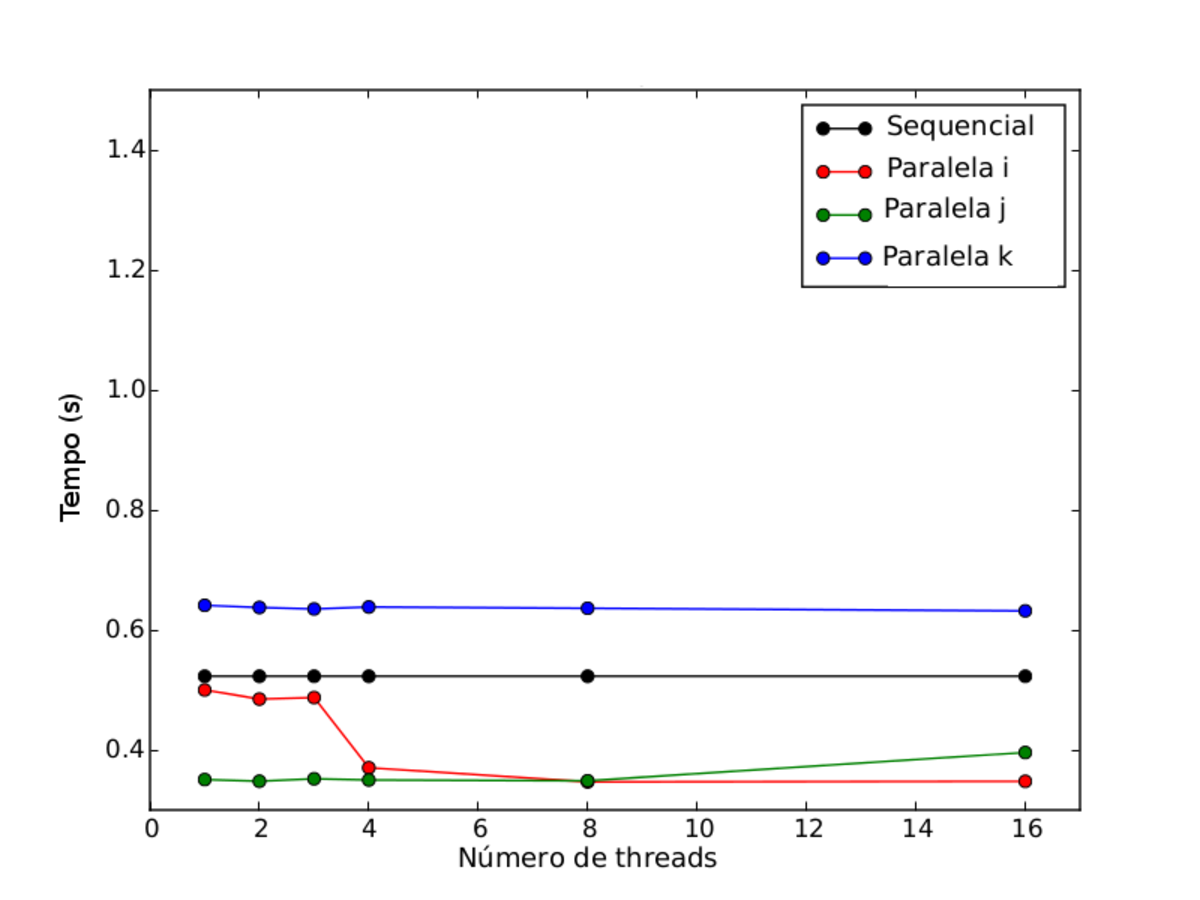
\includegraphics[height=6cm]{Images/corei5co} 
        \caption{Intel Core i5}
        \label{fig:corei5co} 
    \end{subfigure}%
    \begin{subfigure}{.5\textwidth}
        \centering
        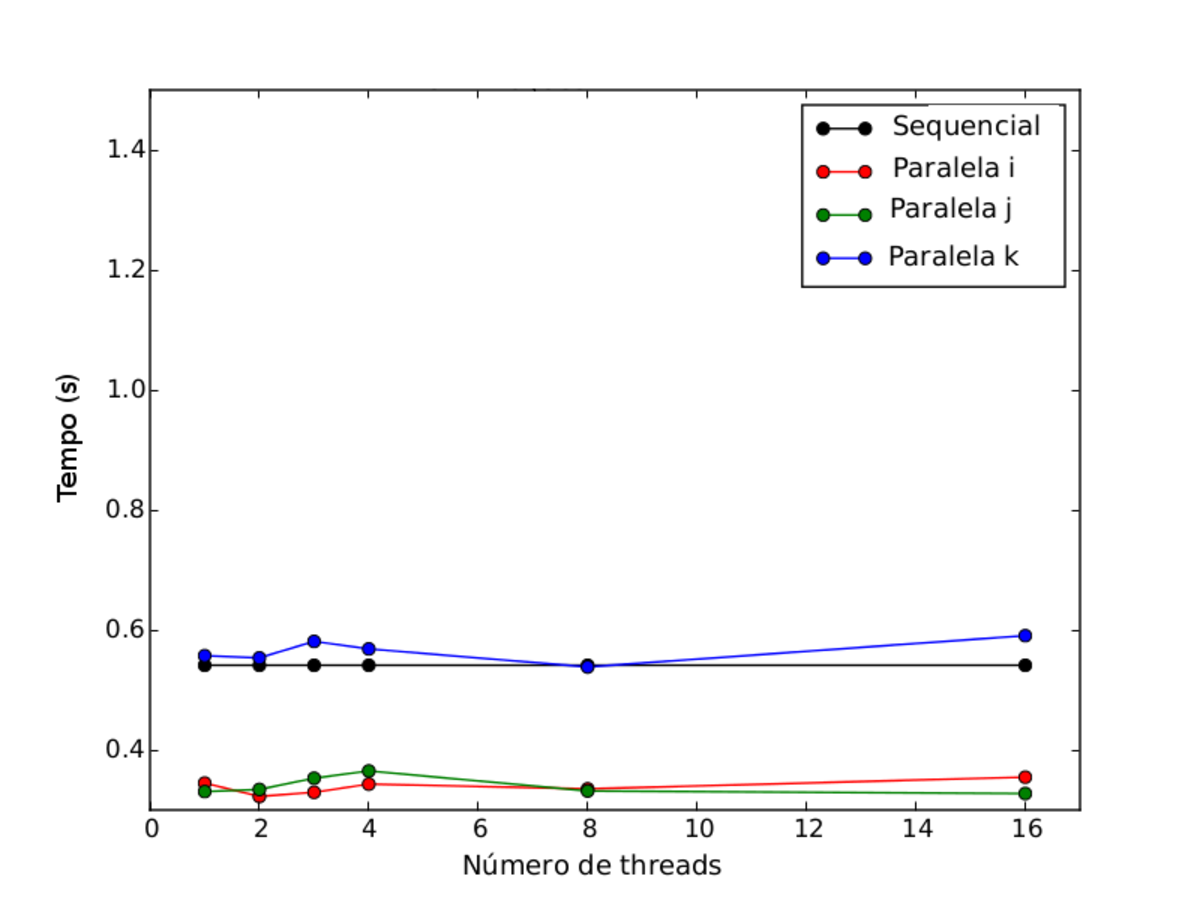
\includegraphics[height=6cm]{Images/xeonco} 
        \caption{Intel Xeon}
        \label{fig:xeonco} 
    \end{subfigure}    
    \caption{Diretivas OpenMP, com otimizações}
    \label{fig:co}
\end{figure} 


TALK STH


Para fazer uma melhor comparação entre os resultados observados nos tempos de execução dos códigos com otmizações de código apresentamos os grafos com um rango menor de tempo.

\begin{figure} 
    \centering
    \begin{subfigure}{.5\textwidth}
        \centering
        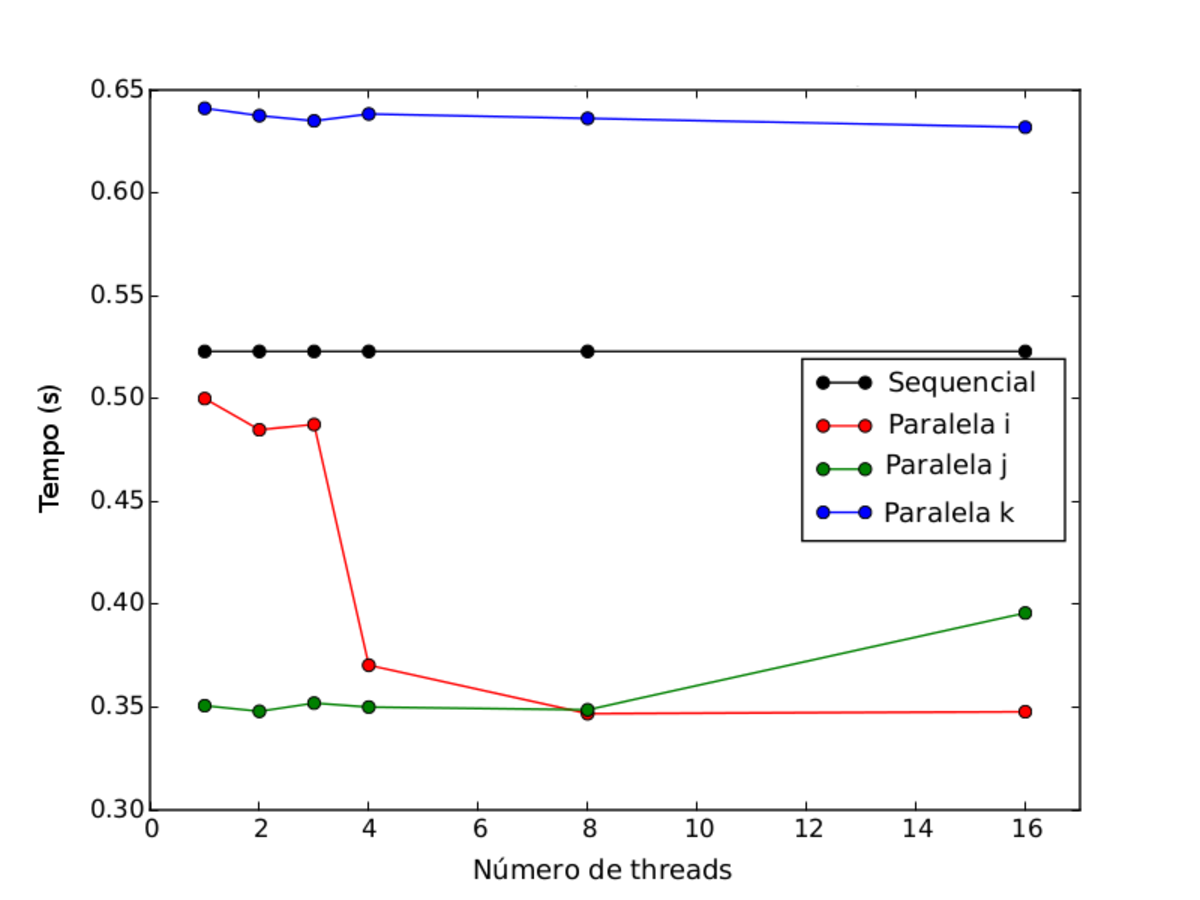
\includegraphics[height=6cm]{Images/corei5cozoom} 
        \caption{Intel Core i5}
        \label{fig:corei5cozoom} 
    \end{subfigure}%
    \begin{subfigure}{.5\textwidth}
        \centering
        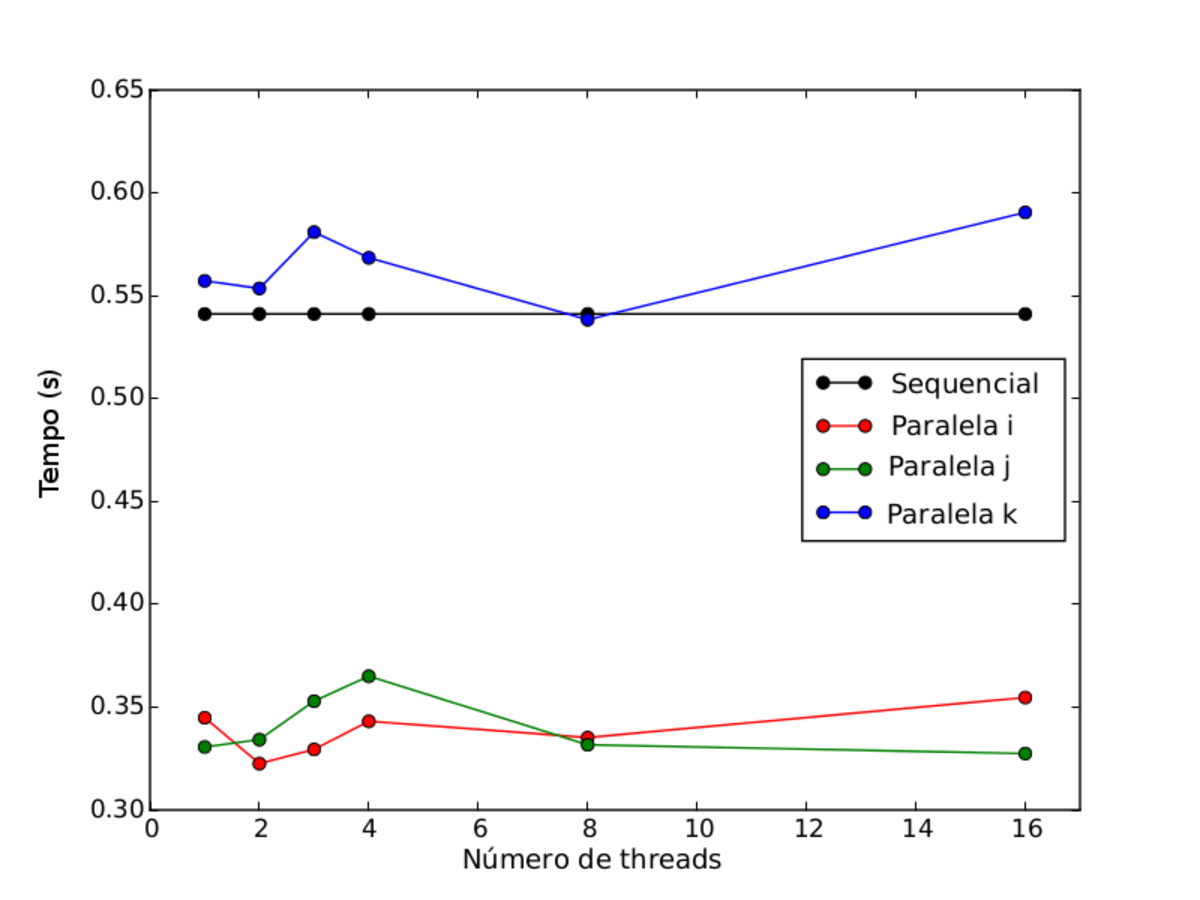
\includegraphics[height=6cm]{Images/xeoncozoom} 
        \caption{Intel Xeon}
        \label{fig:xeoncozoom} 
    \end{subfigure}    
    \caption{Diretivas OpenMP, com otimizações (Zoom)}
    \label{fig:cozoom}
\end{figure} 

TALK STH

\subsection{Conclusões} 

TALK MORE
 
\clearpage 
\section{Conclusões} 
Apresentar as conclusões finais. 
 
\clearpage 
 
\bibliographystyle{plain}   
\bibliography{bibliografia.bib} 
\appendix 
 
\section{Anexo I} 
\label{anex1} 
 
Código do programa mult.c sequencial com trocas para a medição do tempo. 
\begin{verbatim} 
/*
ID: diana.n1
PROG: MultSeqCodeChange
LANG: C++
*/

#include <stdio.h>
#include <assert.h>
#include <stdlib.h>
#include <assert.h>
#include <time.h>
#include "omp.h"

void transpose(int n, long ** m){
	long tmp;
	for (int i = 0; i < n; i++){
		for (int j = i+1; j < n; j++){
			tmp = m[i][j];
			m[i][j] = m[j][i];
			m[j][i] = tmp;
		}
	}	
}

int main(int argc, char **argv) {
	double start, end; 
	start = omp_get_wtime();
	long **a, **b, **c;
    int N = 500;
	
    if (argc == 2) {
      N = atoi (argv[1]);
      assert (N > 0);
    }

    int i,j,k,mul=5;
    long col_sum = N * (N-1) / 2, tmp;
	
		
	a = (long **)malloc (N * sizeof(long *));
	b = (long **)malloc (N * sizeof(long *));
	c = (long **)malloc (N * sizeof(long *));
	for (i=0; i<N; i++) {
	  a[i] = (long *)malloc (N * sizeof(long));
	  b[i] = (long *)malloc (N * sizeof(long));
	  c[i] = (long *)malloc (N * sizeof(long));
	}


	for (i=0; i<N; i++){
	  for (j=0; j<N; j++) {
		a[i][j] = i*mul;
		b[i][j] = i;
		c[i][j] = 0;
	  }
	}

	printf ("Matrix generation finished.\n");         

	transpose(N, b);
	for (i=0; i<N; i++){
	  	for (j=0; j<N; j++){
			tmp = 0;
			for (k=0; k<N; k++){
				tmp += a[i][k] * b[j][k];
			}
			c[i][j] = tmp;
	  	}
	}

	printf ("Multiplication finished.\n");         
	
	for (i=0; i<N; i++)
	  for (j=0; j<N; j++)
		assert ( c[i][j] == i*mul * col_sum);  
    printf ("Test finished.\n");         

	end = omp_get_wtime();
	printf("Time: %lf.\n", end-start);
}
\end{verbatim}
 
Código do programa mult.c com paralelização no laço da variável i. 
\begin{verbatim} 
/*
ID: diana.n1
PROG: MultParalleli
LANG: C++
*/

#include <stdio.h>
#include <assert.h>
#include <stdlib.h>
#include <assert.h>
#include <time.h>
#include "omp.h"

int main(int argc, char **argv) {
	double start, end; 
	start = omp_get_wtime();
    int nthreads, tid, chunk = 10;
	
	long **a, **b, **c;
    int N = 500;
	
    if (argc == 2) {
      N = atoi (argv[1]);
      assert (N > 0);
    }

    int i,j,k,mul=5;
    long col_sum = N * (N-1) / 2;
	
	a = (long **)malloc (N * sizeof(long *));
	b = (long **)malloc (N * sizeof(long *));
	c = (long **)malloc (N * sizeof(long *));
	
	for (i=0; i<N; i++) {
	  a[i] = (long *)malloc (N * sizeof(long));
	  b[i] = (long *)malloc (N * sizeof(long));
	  c[i] = (long *)malloc (N * sizeof(long));
	}

	#pragma omp parallel shared (a,b,c,nthreads, chunk) private (i, j,k,tid) 
	{
		tid = omp_get_thread_num();
		#pragma omp single
			printf("Number threads = %d\n", omp_get_num_threads());

		#pragma omp for schedule(static, chunk)
		for (i=0; i<N; i++){
			for (j=0; j<N; j++) {
				a[i][j] = i*mul;
				b[i][j] = i;
				c[i][j] = 0;
	  		}
		}
		#pragma omp single
			printf ("Matrix generation finished.\n");         
		
		#pragma omp for schedule(static, chunk)
			for (i=0; i<N; i++){
				for (j=0; j<N; j++){
					for (k=0; k<N; k++){
						c[i][j] += a[i][k] * b[k][j];
					}
		  		}
			}
		
		#pragma omp single
			printf ("Multiplication finished.\n");         
	
		#pragma omp for schedule(static, chunk)
			for (i=0; i<N; i++){
			  	for (j=0; j<N; j++){
					assert ( c[i][j] == i*mul * col_sum);  
				}
			}
		#pragma omp single
			printf ("Test finished.\n");         
	}

	end = omp_get_wtime();
	printf("Time: %lf.\n", end-start);
}

\end{verbatim} 
 
Código do programa mult.c com paralelização no laço da variável j. 
\begin{verbatim} 
/*
ID: diana.n1
PROG: MultParallelj
LANG: C++
*/

#include <stdio.h>
#include <assert.h>
#include <stdlib.h>
#include <assert.h>
#include <time.h>
#include "omp.h"

int main(int argc, char **argv) {
	double start, end; 
	start = omp_get_wtime();
    int nthreads, tid, chunk = 10;
	
	long **a, **b, **c;
    int N = 500;
	
    if (argc == 2) {
      N = atoi (argv[1]);
      assert (N > 0);
    }

    int i,j,k,mul=5;
    long col_sum = N * (N-1) / 2;
	
	a = (long **)malloc (N * sizeof(long *));
	b = (long **)malloc (N * sizeof(long *));
	c = (long **)malloc (N * sizeof(long *));
	
	for (i=0; i<N; i++) {
	  a[i] = (long *)malloc (N * sizeof(long));
	  b[i] = (long *)malloc (N * sizeof(long));
	  c[i] = (long *)malloc (N * sizeof(long));
	}

	#pragma omp parallel shared (a,b,c,nthreads, chunk) private (i, j,k,tid) 
	{
		tid = omp_get_thread_num();
		#pragma omp single
			printf("Number threads = %d\n", omp_get_num_threads());

		#pragma omp for schedule(static, chunk)
		for (i=0; i<N; i++){
			for (j=0; j<N; j++) {
				a[i][j] = i*mul;
				b[i][j] = i;
				c[i][j] = 0;
	  		}
		}
		#pragma omp single
			printf ("Matrix generation finished.\n");         
		
		for (i=0; i<N; i++){
			#pragma omp for schedule(static, chunk)
				for (j=0; j<N; j++){
					for (k=0; k<N; k++){
						c[i][j] += a[i][k] * b[k][j];
					}
		  		}
		}
		
		#pragma omp single
			printf ("Multiplication finished.\n");         
	
		#pragma omp for schedule(static, chunk)
			for (i=0; i<N; i++){
			  	for (j=0; j<N; j++){
					assert ( c[i][j] == i*mul * col_sum);  
				}
			}
		#pragma omp single
			printf ("Test finished.\n");         
	}

	end = omp_get_wtime();
	printf("Time: %lf.\n", end-start);
}

\end{verbatim} 
 
Código do programa mult.c com paralelização no laço da variável k. 
\begin{verbatim} 
/*
ID: diana.n1
PROG: MultParallelk
LANG: C++
*/

#include <stdio.h>
#include <assert.h>
#include <stdlib.h>
#include <assert.h>
#include <time.h>
#include "omp.h"

int main(int argc, char **argv) {
	double start, end; 
	start = omp_get_wtime();
    int nthreads, tid, chunk = 10;
	
	long **a, **b, **c;
    int N = 500;
	
    if (argc == 2) {
      N = atoi (argv[1]);
      assert (N > 0);
    }

    int i,j,k,mul=5;
    long col_sum = N * (N-1) / 2;
	long temp;
	
	a = (long **)malloc (N * sizeof(long *));
	b = (long **)malloc (N * sizeof(long *));
	c = (long **)malloc (N * sizeof(long *));
	
	for (i=0; i<N; i++) {
	  a[i] = (long *)malloc (N * sizeof(long));
	  b[i] = (long *)malloc (N * sizeof(long));
	  c[i] = (long *)malloc (N * sizeof(long));
	}

	#pragma omp parallel shared (a,b,c,nthreads, chunk, temp) private (i, j,k,tid)
	{
		tid = omp_get_thread_num();
		#pragma omp single
			printf("Number threads = %d\n", omp_get_num_threads());

		#pragma omp for schedule(static, chunk)
		for (i=0; i<N; i++){
			for (j=0; j<N; j++) {
				a[i][j] = i*mul;
				b[i][j] = i;
				c[i][j] = 0;
	  		}
		}
		#pragma omp single
			printf ("Matrix generation finished.\n");         
		
		for (i=0; i<N; i++){
			for (j=0; j<N; j++){
				#pragma omp single
					temp = 0;
				#pragma omp for schedule(static, chunk) reduction (+:temp) 
					for (k=0; k<N; k++){
						temp += a[i][k] * b[k][j];
					}
				#pragma omp single
					c[i][j] = temp;
		  	}
		}
		
		#pragma omp single
			printf ("Multiplication finished.\n");         
	
		#pragma omp for schedule(static, chunk)
			for (i=0; i<N; i++){
			  	for (j=0; j<N; j++){
					assert ( c[i][j] == i*mul * col_sum);  
				}
			}
		#pragma omp single
			printf ("Test finished.\n");         
	}

	end = omp_get_wtime();
	printf("Time: %lf.\n", end-start);
}

\end{verbatim} 
 
\section{Anexo II} 
\label{anex2} 
 
Código do programa mult.c sequencial com optimizações de código. 
\begin{verbatim} 
/*
ID: diana.n1
PROG: MultSeqCodeChange
LANG: C++
*/

#include <stdio.h>
#include <assert.h>
#include <stdlib.h>
#include <assert.h>
#include <time.h>
#include "omp.h"

void transpose(int n, long ** m){
	long tmp;
	for (int i = 0; i < n; i++){
		for (int j = i+1; j < n; j++){
			tmp = m[i][j];
			m[i][j] = m[j][i];
			m[j][i] = tmp;
		}
	}	
}

int main(int argc, char **argv) {
	double start, end; 
	start = omp_get_wtime();
	long **a, **b, **c;
    int N = 500;
	
    if (argc == 2) {
      N = atoi (argv[1]);
      assert (N > 0);
    }

    int i,j,k,mul=5;
    long col_sum = N * (N-1) / 2, tmp;
	
		
	a = (long **)malloc (N * sizeof(long *));
	b = (long **)malloc (N * sizeof(long *));
	c = (long **)malloc (N * sizeof(long *));
	for (i=0; i<N; i++) {
	  a[i] = (long *)malloc (N * sizeof(long));
	  b[i] = (long *)malloc (N * sizeof(long));
	  c[i] = (long *)malloc (N * sizeof(long));
	}


	for (i=0; i<N; i++){
	  for (j=0; j<N; j++) {
		a[i][j] = i*mul;
		b[i][j] = i;
		c[i][j] = 0;
	  }
	}

	printf ("Matrix generation finished.\n");         

	transpose(N, b);
	for (i=0; i<N; i++){
	  	for (j=0; j<N; j++){
			tmp = 0;
			for (k=0; k<N; k++){
				tmp += a[i][k] * b[j][k];
			}
			c[i][j] = tmp;
	  	}
	}

	printf ("Multiplication finished.\n");         
	
	for (i=0; i<N; i++)
	  for (j=0; j<N; j++)
		assert ( c[i][j] == i*mul * col_sum);  
    printf ("Test finished.\n");         

	end = omp_get_wtime();
	printf("Time: %lf.\n", end-start);
}

\end{verbatim} 
 
Código do programa mult.c com paralelização no laço da variável i com optimizações de código. 
\begin{verbatim} 

/*
ID: diana.n1
PROG: MultParalleliCodeChange
LANG: C++
*/

#include <stdio.h>
#include <assert.h>
#include <stdlib.h>
#include <assert.h>
#include <time.h>
#include "omp.h"

void transpose(int n, long ** m){
	long tmp;
	for (int i = 0; i < n; i++){
		for (int j = i+1; j < n; j++){
			tmp = m[i][j];
			m[i][j] = m[j][i];
			m[j][i] = tmp;
		}
	}	
}

int main(int argc, char **argv) {
	double start, end; 
	start = omp_get_wtime();
    int nthreads, tid, chunk = 10;
	
	long **a, **b, **c;
    int N = 500;
	
    if (argc == 2) {
      N = atoi (argv[1]);
      assert (N > 0);
    }

    int i,j,k,mul=5;
    long col_sum = N * (N-1) / 2, tmp;
	
	a = (long **)malloc (N * sizeof(long *));
	b = (long **)malloc (N * sizeof(long *));
	c = (long **)malloc (N * sizeof(long *));
	
	for (i=0; i<N; i++) {
	  a[i] = (long *)malloc (N * sizeof(long));
	  b[i] = (long *)malloc (N * sizeof(long));
	  c[i] = (long *)malloc (N * sizeof(long));
	}

	#pragma omp parallel shared (a,b,c,nthreads, chunk) private (i, j,k,tid, tmp) 
	{
		tid = omp_get_thread_num();
		
		#pragma omp single
			printf("Number threads = %d\n", omp_get_num_threads());

		#pragma omp for schedule(static, chunk)
		for (i=0; i<N; i++){
			for (j=0; j<N; j++) {
				a[i][j] = i*mul;
				b[i][j] = i;
				c[i][j] = 0;
	  		}
		}
		
		#pragma omp single
			printf ("Matrix generation finished.\n");         
	
		#pragma omp single
			transpose(N, b);

		#pragma omp for schedule(static, chunk)
			for (i=0; i<N; i++){
				for (j=0; j<N; j++){	
					tmp = 0;
					for (k=0; k<N; k++){

						tmp += a[i][k] * b[j][k];
					}
					c[i][j] = tmp;
		  		}
			}
		
		#pragma omp single
			printf ("Multiplication finished.\n");         
	
		#pragma omp for schedule(static, chunk)
			for (i=0; i<N; i++){
			  	for (j=0; j<N; j++){
					assert ( c[i][j] == i*mul * col_sum);  
				}
			}
		#pragma omp single
			printf ("Test finished.\n");         
	}

	end = omp_get_wtime();
	printf("Time: %lf.\n", end-start);
}

\end{verbatim} 
 
Código do programa mult.c com paralelização no laço da variável j com optimizações de código. 
\begin{verbatim} 
/*
ID: diana.n1
PROG: MultParalleljCodeChange
LANG: C++
*/

#include <stdio.h>
#include <assert.h>
#include <stdlib.h>
#include <assert.h>
#include <time.h>
#include "omp.h"

void transpose(int n, long ** m){
	long tmp;
	for (int i = 0; i < n; i++){
		for (int j = i+1; j < n; j++){
			tmp = m[i][j];
			m[i][j] = m[j][i];
			m[j][i] = tmp;
		}
	}	
}

int main(int argc, char **argv) {
	double start, end; 
	start = omp_get_wtime();
    int nthreads, tid, chunk = 10;
	
	long **a, **b, **c;
    int N = 500;
	
    if (argc == 2) {
      N = atoi (argv[1]);
      assert (N > 0);
    }

    int i,j,k,mul=5;
    long col_sum = N * (N-1) / 2, tmp;
	
	a = (long **)malloc (N * sizeof(long *));
	b = (long **)malloc (N * sizeof(long *));
	c = (long **)malloc (N * sizeof(long *));
	
	for (i=0; i<N; i++) {
	  a[i] = (long *)malloc (N * sizeof(long));
	  b[i] = (long *)malloc (N * sizeof(long));
	  c[i] = (long *)malloc (N * sizeof(long));
	}

	#pragma omp parallel shared (a,b,c,nthreads, chunk) private (i,  j, k, tid, tmp) 
	{
		tid = omp_get_thread_num();
		#pragma omp single
			printf("Number threads = %d\n", omp_get_num_threads());

		#pragma omp for schedule(static, chunk)
		for (i=0; i<N; i++){
			for (j=0; j<N; j++) {
				a[i][j] = i*mul;
				b[i][j] = i;
				c[i][j] = 0;
	  		}
		}
		#pragma omp single
			printf ("Matrix generation finished.\n");      

		#pragma omp single
			transpose(N, b);
		
		for (i=0; i<N; i++){
			#pragma omp for schedule(static, chunk)
				for (j=0; j<N; j++){
					tmp = 0;
					for (k=0; k<N; k++){
						tmp += a[i][k] * b[j][k];
					}
					c[i][j] = tmp;
		  		}
		}
		
		#pragma omp single
			printf ("Multiplication finished.\n");         
	
		#pragma omp for schedule(static, chunk)
			for (i=0; i<N; i++){
			  	for (j=0; j<N; j++){
					assert ( c[i][j] == i*mul * col_sum);  
				}
			}
		#pragma omp single
			printf ("Test finished.\n");         
	}

	end = omp_get_wtime();
	printf("Time: %lf.\n", end-start);
}

\end{verbatim} 
 
Código do programa mult.c com paralelização no laço da variável k com optimizações de código. 
\begin{verbatim} 
/*
ID: diana.n1
PROG: MultParallelkCodeChange
LANG: C++
*/

#include <stdio.h>
#include <assert.h>
#include <stdlib.h>
#include <assert.h>
#include <time.h>
#include "omp.h"

void transpose(int n, long ** m){
	long tmp;
	for (int i = 0; i < n; i++){
		for (int j = i+1; j < n; j++){
			tmp = m[i][j];
			m[i][j] = m[j][i];
			m[j][i] = tmp;
		}
	}	
}

int main(int argc, char **argv) {
	double start, end; 
	start = omp_get_wtime();
    int nthreads, tid, chunk = 10;
	
	long **a, **b, **c;
    int N = 500;
	
    if (argc == 2) {
      N = atoi (argv[1]);
      assert (N > 0);
    }

    int i,j,k,mul=5;
    long col_sum = N * (N-1) / 2, tmp;
	
	a = (long **)malloc (N * sizeof(long *));
	b = (long **)malloc (N * sizeof(long *));
	c = (long **)malloc (N * sizeof(long *));
	
	for (i=0; i<N; i++) {
	  a[i] = (long *)malloc (N * sizeof(long));
	  b[i] = (long *)malloc (N * sizeof(long));
	  c[i] = (long *)malloc (N * sizeof(long));
	}

	#pragma omp parallel shared (a,b,c,nthreads, chunk, tmp) private (i, j,k,tid)
	{
		tid = omp_get_thread_num();
		#pragma omp single
			printf("Number threads = %d\n", omp_get_num_threads());

		#pragma omp for schedule(static, chunk)
		for (i=0; i<N; i++){
			for (j=0; j<N; j++) {
				a[i][j] = i*mul;
				b[i][j] = i;
				c[i][j] = 0;
	  		}
		}
		#pragma omp single
			printf ("Matrix generation finished.\n");         
		
		#pragma omp single
			transpose(N, b);

		for (i=0; i<N; i++){
			for (j=0; j<N; j++){
				#pragma omp single
					tmp = 0;
				#pragma omp for schedule(static, chunk) reduction (+:tmp) 
					for (k=0; k<N; k++){
						tmp += a[i][k] * b[j][k];
					}
				#pragma omp single
					c[i][j] = tmp;
		  	}
		}
		
		#pragma omp single
			printf ("Multiplication finished.\n");         
	
		#pragma omp for schedule(static, chunk)
			for (i=0; i<N; i++){
			  	for (j=0; j<N; j++){
					assert ( c[i][j] == i*mul * col_sum);  
				}
			}
		#pragma omp single
			printf ("Test finished.\n");         
	}

	end = omp_get_wtime();
	printf("Time: %lf.\n", end-start);
}
\end{verbatim} 
 
\end{document} 
 
 
 
 
 
